\documentclass{beamer}
\usepackage{tkz-euclide}

% Removes navigation symbols for a cleaner look
\setbeamertemplate{navigation symbols}{}

\begin{document}

\begin{frame}
\frametitle{Construction of Tangents from an External Point}

\centering
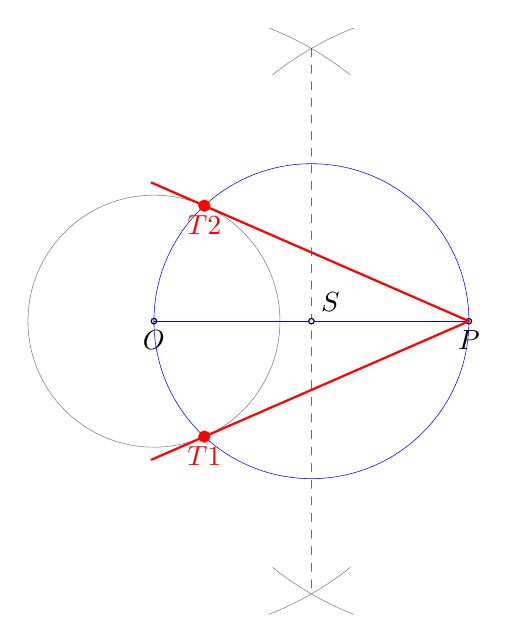
\begin{tikzpicture}[scale=0.8]
    % --- 1. DEFINITIONS (Always calculate these, even if not drawing yet) ---
    \tkzDefPoint(0,0){O}
    \tkzDefPoint(0,2){r}
    \tkzDefPoints{5/0/P}
    
    % Calculate the mediator and midpoint S
    \tkzDefLine[mediator](O,P) \tkzGetPoints{md1}{md2}
    \tkzInterLL(O,P)(md1,md2) \tkzGetPoint{S}
    
    % Calculate the intersection points (Tangents)
    \tkzInterCC(S,P)(O,r) \tkzGetPoints{T1}{T2}

    % --- 2. STATIC ELEMENTS (Visible on all slides) ---
    \tkzDrawCircle(O,r)
    \tkzDrawPoints(O,P)
    \tkzLabelPoints(O,P)

    % --- 3. ANIMATION STEPS ---
    
    % Step 2: Connect O and P
    \onslide<2->{
        \tkzDrawSegment[color=blue](O,P)
    }

    % Step 3: Draw construction arcs (Compass)
    % We use <3-5> so they disappear after step 5 to clean up the drawing
    \onslide<3-5>{
        \tkzCompass[color=gray, length=1.5](P,md1)
        \tkzCompass[color=gray, length=1.5](P,md2)
        \tkzCompass[color=gray, length=1.5](O,md1)
        \tkzCompass[color=gray, length=1.5](O,md2)
    }

    % Step 4: Draw the mediator line
    \onslide<4->{
        \tkzDrawSegment[dashed,color=blue](md1,md2)
        \tkzDrawPoint(S)
        \tkzLabelPoint[above right](S){$S$}
    }

    % Step 5: Draw the Thales Circle
    \onslide<5->{
        \tkzDrawCircle[color=blue](S,P)
    }

    % Step 6: Highlight Intersection Points T1, T2
    \onslide<6->{
        \tkzDrawPoints[color=red, size=4](T1,T2)
        \tkzLabelPoints[color=red](T1,T2)
    }

    % Step 7: Draw the final Tangent Lines
    \onslide<7->{
        \tkzDrawLines[thick, color=red, add=0 and 0.2](P,T1 P,T2)
    }

\end{tikzpicture}
\end{frame}

\end{document}